% ================================================================
% CIS I — Assignment 2: Kinematic Calibration of a Cartesian Robot
% Overleaf-ready report skeleton. Compile with pdfLaTeX + Biber.
%
% EDITING GUIDE
%   (1) Replace all \placeholder{...} text with verified content.
%   (2) Insert real figures into figures/ and use \includegraphics.
%   (3) Cite the precise lecture / handout / literature source.
%   (4) Keep methods, implementation/unit tests, and results distinct.
%   (5) Never replace missing measurements with invented numbers.
% ================================================================
\documentclass[11pt,letterpaper]{article}

% ---------- Typography and page geometry ----------
\usepackage[margin=1in,headheight=16pt]{geometry}
\usepackage[T1]{fontenc}
\usepackage[utf8]{inputenc}
\usepackage{newtxtext,newtxmath}
\usepackage{microtype}
\usepackage{setspace}
\setstretch{1.11}
\usepackage{parskip}
\setlength{\parskip}{5pt}

% ---------- Mathematics, figures and tables ----------
\usepackage{amsmath,mathtools,bm}
\usepackage{graphicx}
\graphicspath{{figures/}}
\usepackage{booktabs,tabularx,multirow,array}
\usepackage{siunitx}
\sisetup{detect-all,per-mode=symbol}
\usepackage{float}
\usepackage{caption}
\captionsetup{font=small,labelfont=bf}
\usepackage{subcaption}
\usepackage{algorithm}
\usepackage{algpseudocode}
\usepackage{xcolor}
\usepackage{titlesec}
\usepackage{fancyhdr}
\usepackage{enumitem}
\usepackage{lastpage}

% ---------- Citations and cross references ----------
\usepackage[backend=biber,style=numeric,sorting=none,maxbibnames=8]{biblatex}
\addbibresource{references.bib}
\usepackage[colorlinks=true,linkcolor=darkblue,citecolor=darkblue,urlcolor=darkblue]{hyperref}
\usepackage[nameinlink,noabbrev]{cleveref}

% ---------- Color palette ----------
\definecolor{darkblue}{HTML}{244B72}
\definecolor{slate}{HTML}{526274}
\definecolor{pale}{HTML}{F2F5F8}
\definecolor{placeholdergray}{HTML}{727E8A}
\definecolor{accent}{HTML}{2B7990}

\titleformat{\section}{\Large\bfseries\color{darkblue}}{\thesection}{0.75em}{}
\titleformat{\subsection}{\large\bfseries\color{darkblue}}{\thesubsection}{0.65em}{}
\titleformat{\subsubsection}{\normalsize\bfseries\color{slate}}{\thesubsubsection}{0.6em}{}
\titlespacing*{\section}{0pt}{2.1ex plus 0.5ex}{0.9ex}
\titlespacing*{\subsection}{0pt}{1.6ex plus 0.3ex}{0.5ex}

\pagestyle{fancy}
\fancyhf{}
\fancyhead[L]{\small\color{slate} CIS I \enspace/\enspace Assignment 2}
\fancyhead[R]{\small\color{slate} Kinematic Calibration}
\fancyfoot[C]{\small\thepage\ of \pageref{LastPage}}
\renewcommand{\headrulewidth}{0.3pt}
\renewcommand{\footrulewidth}{0pt}

% ---------- Project metadata: replace before submission ----------
\newcommand{\coursename}{EN.601.455/655 Computer Integrated Surgery I}
\newcommand{\reporttitle}{Kinematic Calibration of a Cartesian Robot}
\newcommand{\reportsubtitle}{Assignment 2: Design, Mathematical Methods, and Experimental Evaluation}
\newcommand{\teammemberone}{Student 1 Name \quad | \quad JHED ID: \underline{\hspace{1.25in}}}
\newcommand{\teammembertwo}{Student 2 Name \quad | \quad JHED ID: \underline{\hspace{1.25in}}}

% ---------- Notation and reusable placeholders ----------
\newcommand{\R}{\mathbb{R}}
\newcommand{\SO}{\mathrm{SO}(3)}
\newcommand{\SE}{\mathrm{SE}(3)}
\newcommand{\thv}{\bm{\theta}}
\newcommand{\betav}{\bm{\beta}}
\newcommand{\epsv}{\bm{\epsilon}}
\newcommand{\alphav}{\bm{\alpha}}
\newcommand{\Fhat}{\widehat{F}}
\newcommand{\placeholder}[1]{{\color{placeholdergray}\itshape [To complete: #1]}}
\newcommand{\figureplaceholder}[3]{%
  \begin{figure}[htbp]\centering
  \fcolorbox{slate!45}{pale}{\parbox[c][1.35in][c]{0.83\linewidth}{\centering
  \small\color{slate} Figure placeholder\\[4pt]\emph{#1}}}
  \caption{#2}\label{#3}
  \end{figure}}

\begin{document}
\hypersetup{pageanchor=false}
\begin{titlepage}
  \thispagestyle{empty}
  \vspace*{1.1in}
  {\large\bfseries\color{accent} JOHNS HOPKINS UNIVERSITY\par}
  \vspace{0.13in}
  {\normalsize\color{slate}\coursename\par}
  \vspace{0.5in}
  {\color{darkblue}\rule{\textwidth}{1.2pt}\par}
  \vspace{0.22in}
  {\Huge\bfseries\color{darkblue}\reporttitle\par}
  \vspace{0.18in}
  {\Large\color{slate}\reportsubtitle\par}
  \vspace{0.25in}
  {\color{darkblue}\rule{\textwidth}{0.6pt}\par}
  \vspace{0.6in}
  {\large\bfseries Team Members\par}
  \vspace{0.13in}
  \teammemberone\par
  \teammembertwo\par
  \vspace{0.38in}
  {\large\bfseries Academic Integrity Declaration\par}
  \vspace{0.1in}
  ``I (we) have followed the rules in completing this assignment.''\par
  \vspace{0.19in}
  \begin{tabularx}{\linewidth}{@{}X X@{}}
    \rule{0.92\linewidth}{0.35pt} & \rule{0.92\linewidth}{0.35pt}\\
    \small Signature of student 1 & \small Signature of student 2
  \end{tabularx}
  \vfill
  {\color{slate}\today\par}
\end{titlepage}

\pagenumbering{roman}
\setcounter{page}{1}
\section*{Abstract}
\addcontentsline{toc}{section}{Abstract}
\placeholder{A concise summary of the design problem, methodology, calibration-data budget, independent FK/IK results, total time, and primary limitations. Write this last.}

\tableofcontents
\clearpage
\hypersetup{pageanchor=true}
\pagenumbering{arabic}

% ================================================================
\section{Introduction}\label{sec:introduction}
\subsection{Background and Problem Statement}
Accurate robot positioning requires a kinematic model that accounts for departures from nominal geometry and encoder readings. This assignment calibrates a Cartesian robot with three prismatic joints and a three-axis spherical wrist, using an optical tracker and an end-effector calibration body. Base-placement error, axis misalignment, tool-frame error, and systematic joint distortion cause the physical robot to depart from its nominal model. External tracker observations provide the measurements needed to estimate these corrections.

\subsection{Objectives and Performance Requirements}
The assignment asks for improved forward and inverse kinematics over the work volume, with the performance requirements summarized in \cref{tab:requirements} \parencite{cisi_assignment2}.
\begin{table}[htbp]\centering
\caption{Accuracy and execution requirements from the Assignment 2 handout.}\label{tab:requirements}
\begin{tabular}{@{}lll@{}}\toprule
Criterion & Required bound & Evaluation note\\\midrule
Position accuracy (FK and IK) & \SI{0.2}{\milli\metre} & Workspace-level evaluation\\
Orientation accuracy (FK and IK) & \SI{1e-3}{\radian} & Workspace-level evaluation\\
Program execution & \SI{10}{\minute} & Instructor runtime limit\\\bottomrule
\end{tabular}
\end{table}
RMS and maximum position/orientation errors are reported separately, together with the fraction of attempted targets meeting both accuracy bounds. An acceptable average does not establish accuracy at every pose. Simulated acquisition/testing time and wall-clock computation time are recorded separately; the ten-minute program-execution limit must not be confused with the simulator's elapsed-time counter.

\subsection{Summary of the Proposed Approach}
We follow the recommended parameter-estimation route (Method~1): repeated homing establishes joint offsets, individual joint sweeps supply calibration observations, and physically constrained nonlinear least squares fits a corrected geometric model with smooth joint-distortion terms. This avoids a dense six-dimensional calibration grid. Evaluation distinguishes tracker prediction, physical FK accuracy, numerical FK/IK consistency, and executed physical IK accuracy. Seeds 1, 7, and 61 are calibrated independently, with ordinary-workspace and stress-test results kept separate. Hidden simulator values are used only for evaluation; the provided inverse solver is retained so its numerical limitations can be distinguished from forward-model accuracy.

% ================================================================
\section{System Design and Calibration Setup}\label{sec:design}
\subsection{Robot and Optical Tracker}
The first three joints translate the wrist center along the nominal base axes; the final three rotate a spherical wrist. The joint ranges and speed limits are listed in \cref{tab:joint_limits}. Motion time includes acceleration-limited travel and \SI{0.05}{\second} settling, making wrist travel particularly expensive.
\begin{table}[htbp]\centering
\caption{Joint limits and maximum speeds used in calibration.}\label{tab:joint_limits}
\begin{tabular}{@{}lll@{}}\toprule
Joints & Permitted range & Maximum speed\\\midrule
$1,3$ & $[0,600]$ mm & \SI{50}{\milli\metre\per\second}\\
$2$ & $[-300,300]$ mm & \SI{50}{\milli\metre\per\second}\\
$4,5$ & $[-3\pi/4,3\pi/4]$ rad & \SI{0.1}{\radian\per\second}\\
$6$ & $[-\pi,\pi]$ rad & \SI{0.1}{\radian\per\second}\\\bottomrule
\end{tabular}
\end{table}

The tracker has a square viewing frustum extending from \SI{1000}{\milli\metre} to \SI{2200}{\milli\metre} along its local $+z$ axis. Marker measurements include independent per-coordinate noise with standard deviation \SI{0.1}{\milli\metre} and spatially varying systematic error. Camera-pose jiggle is disabled by the assignment, which does not make the marker observations noiseless. Each snapshot costs \SI{0.03}{\second} of simulated time.

\subsection{Coordinate Frames and Nominal Geometry}
The nominal robot model is expressed as \parencite{cisi_assignment2,cisi_frames}:
\begin{equation}\label{eq:nominal_fk}
F_{BE}^{\mathrm{nom}}(\thv)
=F_c(\theta_1,\theta_2,\theta_3)\,F_{cw}\,F_w(\theta_4,\theta_5,\theta_6)\,F_{we}.
\end{equation}
Let $W$, $T$, $B$, and $E$ denote workspace, tracker, robot-base, and end-effector frames. The convention $F_{AB}={}^AT_B$ maps coordinates from $B$ into $A$. In \cref{eq:nominal_fk}, $F_c=\operatorname{Trans}(\theta_1,\theta_2,\theta_3)$, $F_{cw}=\operatorname{Trans}(500,0,0)$, and $F_{we}=\operatorname{Trans}(100,0,0)$, with translations in millimeters; $F_w$ applies the ordered rotations $R_x(\theta_4)R_y(\theta_5)R_z(\theta_6)$. Rotations are embedded in homogeneous transformations. The tracker-frame prediction is
\begin{equation}\label{eq:tracker_chain}
\widehat F_{TE}(\thv)=\widehat F_{TB}\,F_{BE}(\thv),
\qquad F_{TB}=F_{WT}^{-1}F_{WB}.
\end{equation}
The estimated base-to-tracker transform is applied once on the left; the nominal or corrected $F_{BE}$ describes the robot's internal kinematics.

\subsection{Calibration Marker Body Design}
Four markers form a regular tetrahedron centered at the end-effector origin, with coordinates given in \cref{tab:markers}. Each marker has radius $37.5\sqrt{3}=\SI{64.95}{\milli\metre}$, below the \SI{75}{\milli\metre} limit. This symmetric, noncoplanar layout spreads the observations in three dimensions and avoids favoring one rotational direction. The special calibration body's geometry is exact under the TA API, and its frame coincides with $E$. Therefore, no marker-manufacturing refinement or separate marker-to-tool transform is estimated.
\begin{table}[htbp]\centering
\caption{Calibration marker coordinates in the end-effector frame.}\label{tab:markers}
\begin{tabular}{@{}cccc@{}}\toprule
Marker & $x$ (mm) & $y$ (mm) & $z$ (mm)\\\midrule
$m_1$ & $37.5$ & $37.5$ & $37.5$\\
$m_2$ & $37.5$ & $-37.5$ & $-37.5$\\
$m_3$ & $-37.5$ & $37.5$ & $-37.5$\\
$m_4$ & $-37.5$ & $-37.5$ & $37.5$\\\bottomrule
\end{tabular}
\end{table}

\subsection{Camera Placement and Visibility Analysis}
The tracker frame coincides with the workspace frame and looks along $+z$. The chosen approximate robot-base pose is
\begin{equation}\label{eq:scene_placement}
F_{WT}=I,\qquad F_{WB}^{\mathrm{approx}}=\operatorname{Trans}(-800,0,1300),
\end{equation}
with translation coordinates in millimeters. Including the fixed base-to-wrist offset, nominal wrist-center travel is $x,y\in[-300,300]$ mm and $z\in[1300,1900]$ mm, centered at $(0,0,1600)$ mm.

For any wrist orientation, the tool length and marker radius bound the distance from wrist center to a marker by $\rho=100+64.95=\SI{164.95}{\milli\metre}$. Thus a conservative marker envelope is
\begin{equation}\label{eq:marker_envelope}
|x|,|y|\leq\SI{464.95}{\milli\metre},\qquad
z\in[1135.05,2064.95]\ \mathrm{mm}.
\end{equation}
The frustum half-width is $h(z)=500+(500/1200)(z-1000)$, with $z$ and $h$ in millimeters. At the envelope's nearest depth, $h=\SI{556.27}{\milli\metre}$, giving at least \SI{91.32}{\milli\metre} lateral clearance and approximately \SI{135.05}{\milli\metre} near/far clearance. This bound covers the complete nominal joint range, including rotations between sampled poses. It is a nominal geometric result, not a guarantee under every unknown physical perturbation.

\begin{figure}[htbp]\centering
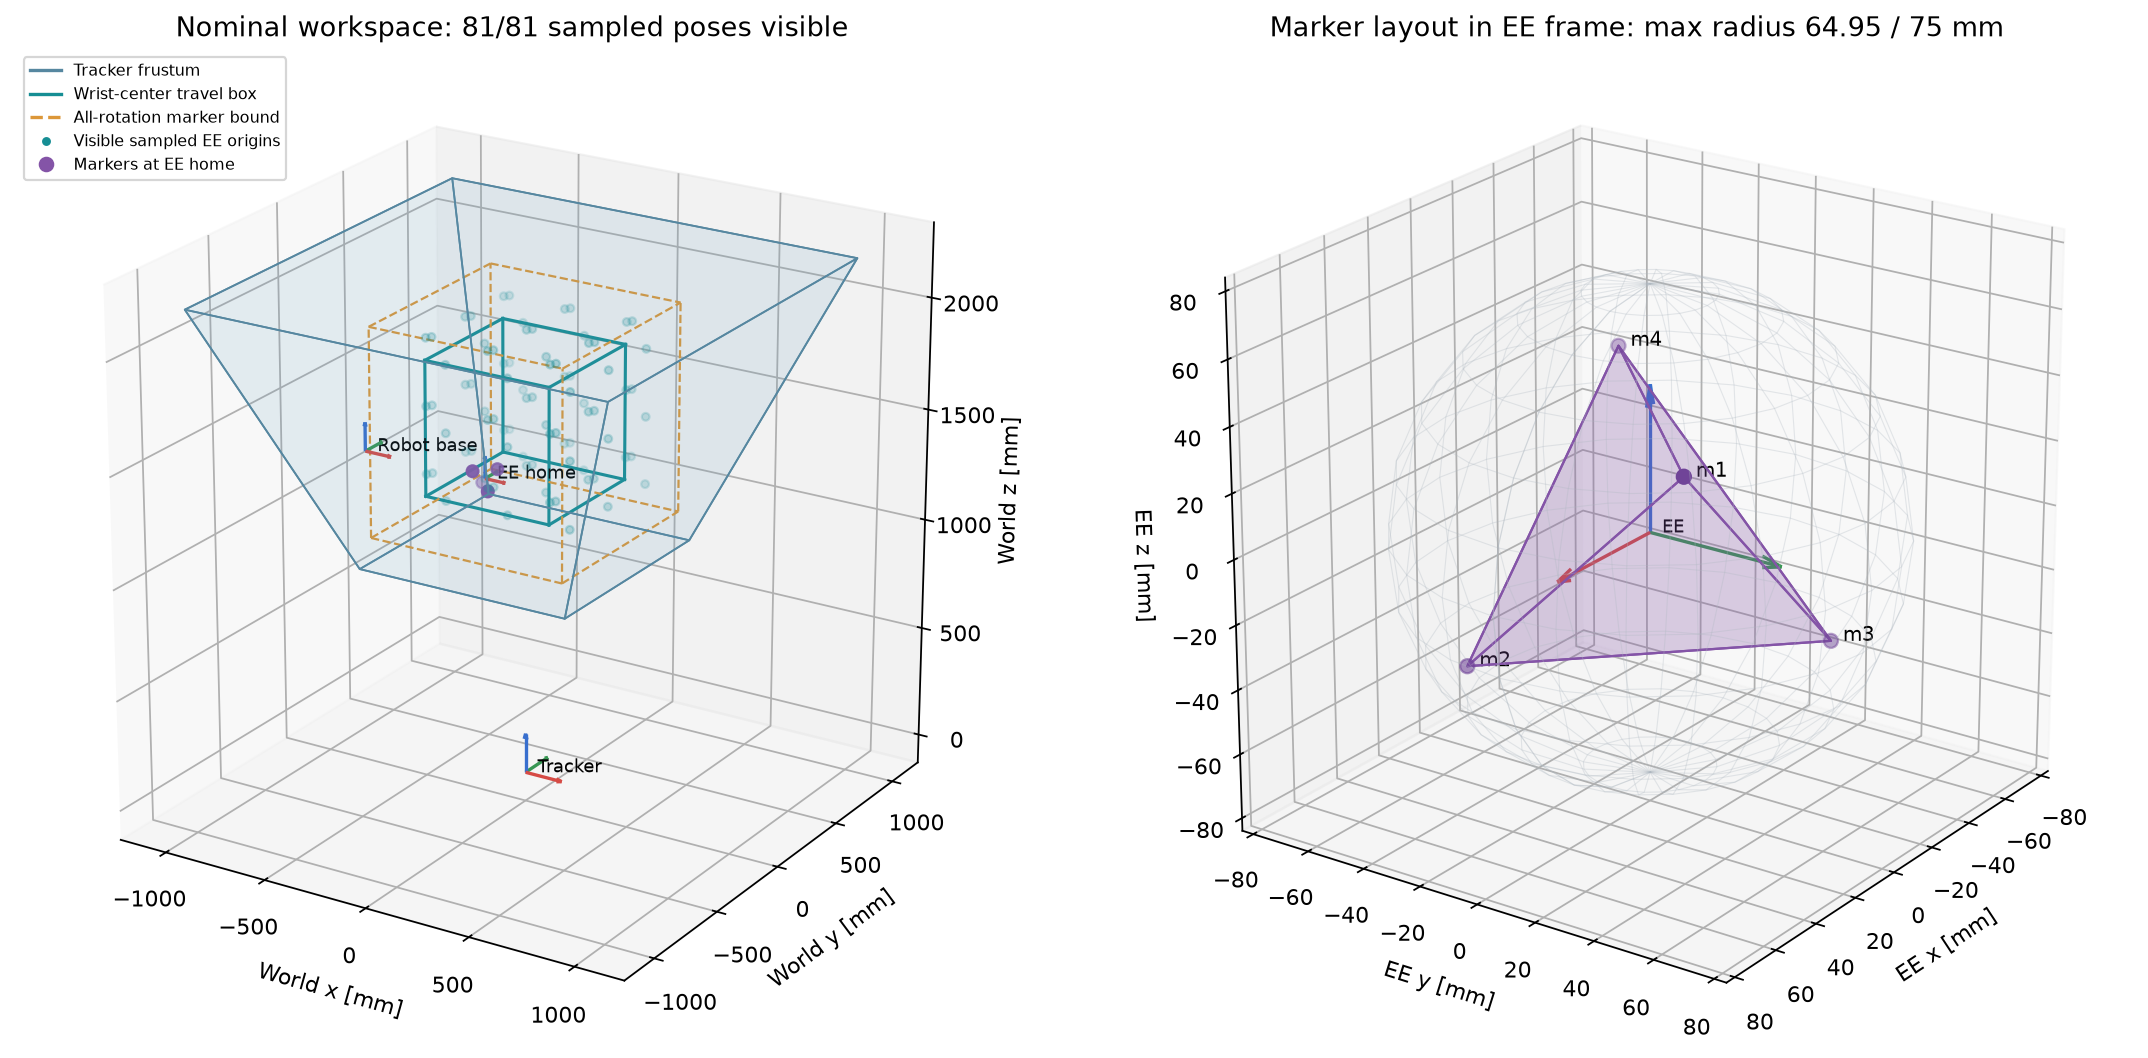
\includegraphics[width=\linewidth]{workspace_design.png}
\caption{Nominal scene placement and conservative marker envelope (left), and tetrahedral marker layout in end-effector coordinates (right). The plot checks visibility, not calibrated positioning accuracy.}\label{fig:visibility}
\end{figure}

\subsection{Design Verification and Unit Tests}
Design checks require all markers to satisfy the radius constraint, the centered layout to span three dimensions, every planned command to satisfy joint limits, and every nominal marker to remain in the tracker frustum. All 81 initial visualization poses pass visibility checks. An additional sweep using three values for each linear joint and five for each wrist joint retains all markers at $3^3\times5^3=3375/3375$ nominal poses. These numerical checks support the analytic envelope; they do not establish calibration accuracy.

The acquisition setup uses five homings, ten mixed baseline observations, and 765 calibration observations across 69 distinct single-axis configurations. Eleven re-commanded readings per configuration, plus return-reference readings, renew both tracker and robot repeatability noise. Each valid tracker frame is paired with its settled encoder reading; missing observations are not replaced by stale data. The same design is applied independently to each seed, costing approximately \SIrange{554.03}{554.06}{\second} simulated time including homing and baseline measurements. Sampling-density, repetition, and estimator derivations are developed in \cref{sec:math}.

% ================================================================
\section{Mathematical Methods}\label{sec:math}
\subsection{Rigid Frames and Pose-Error Metrics}
\placeholder{Derive rigid-frame composition and inversion and define the signed orientation/position residual. Cite the exact relevant lecture pages.}
A general relative-pose error may be written as
\begin{equation}\label{eq:pose_error}
\Delta F=F_{\mathrm{reference}}^{-1}F_{\mathrm{prediction}}.
\end{equation}
\placeholder{Explain the axis--angle / rotation-logarithm representation and the translation-error metric, including units and frame convention.}

\subsection{Point Registration and Averaging of Frames}
\placeholder{Present the least-squares rigid-registration objective, rotation constraint, and your frame-averaging method. Explain the relationship to the class material.}

\subsection{Homing and Estimation of the Base Frame}
\placeholder{Derive the sign of the repeated-home encoder correction, its random-noise reduction, and the base transform estimate from observed versus nominal end-effector poses.}

\subsection{Calibration Sampling Density and Measurement Uncertainty}
\placeholder{Derive the combined robot-distortion/tracker-gradient slope, the 1D sweep interpolation bound, wrist spacing, repeated-reading estimate, and assumptions/limitations. Distinguish hard specification bounds from chosen error allocations.}
\begin{equation}\label{eq:interp}
\big\|e_{\mathrm{interp}}\big\|\le \frac{Lh}{2}.
\end{equation}
\placeholder{Explain why this is a one-dimensional bound along each single-joint sweep rather than a global 3D guarantee.}

\subsection{Parameterization of the Improved Kinematic Model}
\placeholder{Define the 34-parameter representation: base-frame correction, axis tilts, tool correction, and joint distortion. Define scales, signs, home anchoring, and gauge choice.}

\subsection{Constrained Nonlinear Least Squares}
\placeholder{Derive the six-dimensional signed residual, units/weights, least-squares objective, parameter scaling, and full-interval physical distortion constraints. Describe solver selection and convergence criteria.}
\begin{equation}\label{eq:least_squares}
\widehat{\betav}=\underset{\betav\in\mathcal C}{\operatorname{argmin}}
\sum_{j=1}^{N}\left\|\bm r_j(\betav)\right\|_2^2,
\end{equation}
where $\mathcal C$ denotes the admissible parameter set.

\subsection{Jacobian Rank and Parameter Identifiability}
\placeholder{Explain numerical differentiation, SVD, the redundant base-axis gauge, and weak but non-null parameter directions; clearly separate identifiability from prediction quality.}

\subsection{Inverse Kinematics and Numerical Limitations}
\placeholder{Summarize the provided numerical IK formulation, its use of improved FK, and known singularity, joint-limit, and angle-wrapping limitations. State explicitly if the original TA implementation was retained.}

% ================================================================
\section{Algorithmic Approach and Implementation}\label{sec:implementation}
\subsection{System Architecture and End-to-End Workflow}
\placeholder{Describe module responsibilities and the caller--callee/data-flow relationships from marker design through evaluation. Do not copy implementation source line-by-line.}
\figureplaceholder{Program/module call hierarchy or calibration pipeline}{Major data and control flow through the calibration program.}{fig:pipeline}

\subsection{Error Metrics, Registration, and Frame Reduction}
\subsubsection{Implementation}
\placeholder{Give concise pseudocode and input/output shapes for core Step 4--5 operations, including corner cases.}
\subsubsection{Unit Tests}
\placeholder{Describe synthetic known-value tests, numerical tolerance and regression outcomes for metrics and registration.}

\subsection{Homing, Pose Planning, and Data Collection}
\subsubsection{Implementation and Pseudocode}
\placeholder{Explain repeated homing, ordered one-axis sweeps, tracker visibility checks, pairing of encoder/Frame observations, repeated commands, and simulated-time accounting.}
\begin{algorithm}[htbp]
\caption{Calibration-data acquisition: algorithmic outline only}\label{alg:acquisition}
\begin{algorithmic}[1]
  \State $\mathcal D\gets\emptyset$
  \State $\mathcal P\gets\Call{PlanCalibrationPoses}{\text{robot, tracker, target accuracy}}$
  \For{each commanded configuration $\thv$ in $\mathcal P$}
    \State \Call{MoveJoints}{$\thv$}
    \State Acquire encoder state and tracker observation
    \If{a valid marker-body observation exists}
      \State Append paired encoder/observed-frame record to $\mathcal D$
    \EndIf
  \EndFor
  \State \Return $\mathcal D$ and measured simulated acquisition time
\end{algorithmic}
\end{algorithm}
\subsubsection{Unit Tests}
\placeholder{Describe visibility, limits, excitation, time accounting, missing observations, and home-sign tests.}

\subsection{Improved Kinematics and Parameter Fitting}
\subsubsection{Implementation and Pseudocode}
\placeholder{Describe parameter initialization, forward model, gauge handling, constrained optimization, checkpointing, and parameter report.}
\subsubsection{Unit Tests}
\placeholder{Describe nominal recovery, perturbation tests, synthetic noiseless parameter fitting, SVD-rank checks, physical-bound checks, and held-out prediction tests.}

\subsection{Forward and Inverse Kinematics Evaluation}
\subsubsection{Implementation}
\placeholder{Distinguish the fixed Step 9 grid, physical Step 10 move-based tests, tracker measurement residuals, and ground-truth reporting-only oracle.}
\subsubsection{Unit Tests and Numerical Edge Cases}
\placeholder{Include FK/IK round trips, limit/singularity cases, documented exceptions or expected failures, and non-TODO TA test outcomes. Avoid claiming that expected failures passed.}

\subsection{Reproducibility and Execution Procedure}
\placeholder{Specify environment, random seeds, saved data, experiment commands, implementation versions, and how to reproduce figures without accidentally rerunning expensive acquisition.}

% ================================================================
\section{Experimental Results and Evaluation}\label{sec:results}
\subsection{Protocols, Metrics, and Random Seeds}
\placeholder{Define training vs held-out configurations, official vs supplemental tests, individual-move results vs averaged tracker observations, and calibration independence across seeds.}

\subsection{Calibration Baseline and Estimated Parameters}
\placeholder{Present the pre-calibration baseline, after-fit residuals, parameter angles/offsets/scales and full-range bound compliance. State which parameters depend on gauge.}
\begin{table}[htbp]\centering
\caption{Template for nominal and calibrated performance. Fill only from final verified results.}\label{tab:main_accuracy}
\begin{tabular}{@{}lcccc@{}}\toprule
& \multicolumn{2}{c}{Position (mm)} & \multicolumn{2}{c}{Orientation (rad)}\\
\cmidrule(lr){2-3}\cmidrule(l){4-5}
Method & RMS & Maximum & RMS & Maximum\\\midrule
Nominal FK & --- & --- & --- & ---\\
Improved FK & --- & --- & --- & ---\\
Nominal IK & --- & --- & --- & ---\\
Improved IK & --- & --- & --- & ---\\\bottomrule
\end{tabular}
\end{table}

\subsection{Forward Kinematics Accuracy}
\placeholder{Report fixed grid, per-pose pass rate, RMS/max/percentiles, comparisons, and genuinely held-out analysis. Do not confuse pose accuracy with model-fit residuals.}
\figureplaceholder{FK position and orientation error CDFs with target lines}{Cumulative FK-error distributions for nominal and improved models.}{fig:fk_cdf}

\subsection{Inverse Kinematics Accuracy}
\placeholder{Report how target poses were selected, commanded joint solutions, executed-move errors, failure counts, and per-target time. Distinguish model consistency from physical placement.}
\figureplaceholder{IK position and orientation error distributions with target lines}{Physical IK accuracy over the evaluation target set.}{fig:ik_cdf}

\subsection{Random Workspace and Multi-Seed Testing}
\placeholder{Report new continuous configurations and independent re-calibrations for other seeds only if actually performed; state seed count and sample counts.}
\figureplaceholder{Error versus position in the work volume}{Spatial distribution of independent end-effector position errors.}{fig:workspace_error}

\subsection{Joint Limits and Wrist Singularities}
\placeholder{Present separate stress-test statistics, numerical IK limitations, and qualitative failure classification. Distinguish these from the official test protocol.}

\subsection{Runtime and Measurement Efficiency}
\placeholder{Report robot-motion time, tracker sampling time, fitting wall-clock time, complete program wall-clock time, and evaluation simulated time. Explain whether a repeated test is included.}
\figureplaceholder{Calibration and evaluation time breakdown}{Time cost of calibration and independent testing; show distinct simulated and wall-clock measures.}{fig:timing}

% ================================================================
\section{Discussion}\label{sec:discussion}
\subsection{Accuracy, Observability, and Physical Plausibility}
\placeholder{Interpret the improvements and remaining error floor; discuss systematic tracker bias, repeatability, parameter coupling, and model mismatch.}
\subsection{Design Trade-offs and Limitations}
\placeholder{Explain the measurement-time-versus-accuracy trade-off, polynomial versus interpolation mismatch, numerical IK limitations, and limits on generalization.}
\subsection{Possible Improvements}
\placeholder{Only suggest modifications supported by an observed limitation or a reasoned analysis.}

\section{Conclusion}\label{sec:conclusion}
\placeholder{Summarize the final independently verified accuracy, calibration cost, central technical contributions, and key limitations.}

% ================================================================
\clearpage
\printbibliography[heading=bibintoc,title={References}]

\appendix
\section{AI Tools and Development Assistance}\label{app:ai}
\placeholder{Identify every AI/development tool used, the purpose and scope of its contribution, how its output was reviewed, and the prompts used. Include the exact prompts or an appropriately organized prompt log as required by the course policies. Do not invent tool use.}

\section{Team Contributions}\label{app:team}
\placeholder{State who designed, implemented, tested, wrote and reviewed each component; name both collaborators accurately.}

\section{Additional Tables, Tests, and Derivations}\label{app:additional}
\placeholder{Place detailed per-seed tables, extended test matrices, full parameter lists, or longer mathematical derivations here only when they add evidence without interrupting the main narrative.}

\end{document}
